\chapter{Schur Polynomials}

Consider the following two representations of \(\sym_n\):
\begin{itemize}
    \item The trivial representation \(1 \colon \sym_n \to \GL_1(\complexes)\) given by \(\sigma \mapsto 1\).
    \item The sign representation \(\sign \colon \sym_n \to \GL_1(\complexes)\) given by \(\sigma \mapsto \sign(\sigma)\).
\end{itemize}

Consider any representation \(\phi \colon  \sym_n \to \GL_1(\complexes)\).
Let \(i \in \interval{n-1}\).
Then,
\begin{equation}
    \phi(\eltr{i}) = \phi(\tau \eltr{1} \tau^{-1}) = \phi(\tau) \phi(\eltr{1}) \phi(\tau)^{-1} = \phi(\eltr{1}),
\end{equation}
for some \(\tau \in \sym_n\).
Thus, \(\phi(\eltr{i})\) is independent of \(i\).
Moreover, \(\phi(\eltr{i})^2 = \phi(\eltr{i}^2) = \phi(\operatorname{id}) = 1\), hence \(\phi(\eltr{i}) = \pm 1\), for all \(i \in \interval{n-1}\).
If \(\phi(\eltr{i}) = 1\) for all \(i \in \interval{n-1}\), then \(\phi = 1\).
If \(\phi(\eltr{i}) = -1\) for all \(i \in \interval{n-1}\), then \(\phi = \sign\).

Therefore, the only irreducible representations of \(\sym_n\) of dimension \(1\) are the trivial representation and the sign representation.

Suppose \(\rho \colon \sym_n \to \GL(V)\) is a representation of \(S_n\).
The \vocab{invariants} of \(\rho\) are the elements \(v \in v\) such that
\begin{equation}
    \rho(w) v = 1(w) v, 
\end{equation}
for all \(w \in S_n\), where \(1\) denotes the trivial representation.
We can alternatively call these elements \vocab{\(1\)-isotypic elements}.
Let \(\Inv(V)\) denote the set of \(1\)-isotypic elements of \(\rho \colon S_n \to \GL(V)\).

We can replace the trivial representation with the sign representation.

The \vocab{\(\sign\)-isotypic elements} of \(\rho\) are the elements \(v \in V\) such that
\begin{equation}
    \rho(w) v = \sign(w) v,
\end{equation}
for all \(w \in S_n\).
Let \(\Alt(V)\) denote the set of \(\sign\)-isotypic elements of \(\rho \colon S_n \to \GL(V)\).

\begin{proposition}
    Let \(\rho \colon S_n \to \GL(V)\) be a representation of \(S_n\).
    Then, \(\Alt(V)\) is a subspace of \(V\).
\end{proposition}

\begin{definition}[Direct sum of representations]
    If \(\rho_1 \colon S_n \to \GL(V_1)\) and \(\rho_2 \colon S_n \to \GL(V_2)\) are representations of \(S_n\),
    then the \vocab{direct sum} of \(\rho_1\) and \(\rho_2\) is the representation \(\rho_1 \oplus \rho_2 \colon S_n \to \GL(V_1 \oplus V_2)\) given by
    \begin{equation}
        (\rho_1 \oplus \rho_2)(w) = \rho_1(w) \oplus \rho_2(w),
    \end{equation}
    for all \(w \in S_n\).
\end{definition}

Much more interesting than adding two representations to get a third,
is to start with a representation and decompose it into a direct sum of other representations.

\begin{theorem}
    Let \(\rho \colon S_n \to \GL(V)\) be a representation of \(S_n\).
    Then, \(V = \Inv(V) \oplus \Alt(V) \oplus W\), for some \(W \subset V\),
    and 
    \begin{equation}
        \rho = 1_{\Inv(V)} \oplus \sign_{\Alt(V)} \oplus \rho|_W.
    \end{equation}
\end{theorem}

We saw that, if \(V\) is an algebra, then \(\Inv(V)\) is a subalgebra of \(V\).
However, this is not the case for \(\Alt(V)\).
Suppose \(a \in \Alt(V)\).
Then \(w \cdot a^2 = (w \cdot a) (w \cdot a) = \sign(w)^2 a^2 = a^2\), for all \(w \in S_n\), which is not always equal to \(\sign(w) a^2\) (for \(n \geq 2\)).
Something can be salvaged from this situation.

\begin{theorem} \label{thm:inv-alt-subalgebra}
    Let \(V\) be an algebra.
    Let \(\rho \colon S_n \to \Aut(V)\) be a representation of \(S_n\).
    Consider the subspace \(\Inv(V) \oplus \Alt(V)\) of \(V\).
    Then, \(\Inv(V) \oplus \Alt(V)\) is a subalgebra of \(V\).
\end{theorem}

The proof of Theorem~\ref{thm:inv-alt-subalgebra} follows from Theorem~\ref{thm:inv-alt-super}.

\begin{definition}[\(G\)-graded algebra]
    A \vocab{\(G\)-graded algebra} is an algebra \(V\) together with a direct sum decomposition
    \begin{equation}
        V = \bigoplus_{g \in G} V_g,
    \end{equation}
    such that \(ab \in V_{gh}\), for all \(a \in V_g\) and \(b \in V_h\).
\end{definition}

A \vocab{superalgebra} is a \(\mathbb{Z}_2\)-graded algebra.

\begin{theorem} \label{thm:inv-alt-super}
    Let \(V\) be an algebra.
    Let \(\rho \colon S_n \to \Aut(V)\) be a representation of \(S_n\).
    Consider the subspace \(\Inv(V) \oplus \Alt(V)\) of \(V\).
    Then, \(\Inv(V) \oplus \Alt(V)\) is a superalgebra with parts \(\Inv(V)\) and \(\Alt(V)\).
\end{theorem}

\begin{proof}
    Let \(a \in \Inv(V)\) and \(b \in \Inv(V)\).
    Then, \(w \cdot (ab) = (w \cdot a) (w \cdot b) = a b\), for all \(w \in S_n\).
    Thus, \(ab \in \Inv(V)\).
    Let \(a \in \Inv(V)\) and \(b \in \Alt(V)\).
    Then, \(w \cdot (ab) = (w \cdot a) (w \cdot b) = (\sign(w) a) b = \sign(w) a b\), for all \(w \in S_n\).
    Thus, \(ab \in \Alt(V)\).
    Let \(a \in \Alt(V)\) and \(b \in \Alt(V)\).
    Then, \(w \cdot (ab) = (w \cdot a) (w \cdot b) = \sign(w)^2 a b = a b\), for all \(w \in S_n\).
    Thus, \(ab \in \Inv(V)\).

    Therefore, \(\Inv(V) \oplus \Alt(V)\) is a subalgebra of \(V\),
    and \(\Inv(V) \oplus \Alt(V)\) is a superalgebra with parts \(\Inv(V)\) and \(\Alt(V)\).
\end{proof}

Now, apply this with \(\mathcal{A} = \rationals[x_1, x_2, \ldots, x_n]\),
and the action \(\rho \colon S_n \to \Aut(\mathcal{A})\) given by
permuting the variables.
The \(\sign\)-isotypic elements of \(\mathcal{A}\) are are the \vocab{alternating polynomials},
denoted by \(\AltPoly(n)\) or \(v_n\Sym(n)\).

For example,
\begin{equation}
    x_1^2x_2 - x_2^2x_1 + x_2^2x_3 - x_3^2x_2 + x_3^2x_1 - x_1^2x_3 \in \AltPoly(3).
\end{equation}

\begin{lemma}
Let \(p \in \AltPoly(n)\).
Let \(\alpha\) be a composition of length \(n\).
Assume that \(\alpha_i = \alpha_j\) for some distinct \(i, j \in \interval{n}\).
Then, the coefficient of \(x^\alpha\) in \(p\) is zero.
\end{lemma}

\begin{proof}
    We compute that     
    \begin{equation}
        [x^\alpha] p = [x^alpha] (- \eltr{i, j} \cdot p) = - [x^\alpha] p,
    \end{equation}
    which implies that \([x^\alpha] p = 0\).
\end{proof}

\begin{definition}[Vandermonde polynomial]
    Define the \vocab{\(n\)\textsuperscript{th} Vandermonde polynomial} to be
    \begin{equation}
        v_n = \prod_{1 \leq i < j \leq n} (x_j - x_i) \in \AltPoly(n).
    \end{equation}
\end{definition}

\begin{lemma} \label{lem:vandermonde-divides-alt}
    Let \(p \in \AltPoly(n)\).
    Then, \(v_n \mid p\).
\end{lemma}

\begin{proof}
    Let \(i < j\) in \(\interval{n}\).
    If we specialize \(p\) by setting \(x_i = x_j\), then \(p \mapsto 0\).
    Therefore, \(x_i - x_j \mid p\).
    Since this holds for all \(i < j\), we have \(v_n \mid p\).
\end{proof}

\begin{lemma} \label{lem:vandermonde-times-sym-is-alt}
    Let \(p \in \AltPoly(n)\).
    Then, \(\frac{p}{v_n} \in \Sym(n)\).
\end{lemma}

\begin{proof}
    Let \(p \in \AltPoly(n)\).
    Then, \(p = v_n q\), for some \(q \in \rationals[x_1, x_2, \ldots, x_n]\),
    by Lemma~\ref{lem:vandermonde-divides-alt}.
    Since \(p, v_n \in \AltPoly(n)\),
    we have \(w \cdot p = \sign(w) p\) and \(w \cdot v_n = \sign(w) v_n\), for all \(w \in S_n\).
    Thus, \(w \cdot q = q\), for all \(w \in S_n\), and consequently, \(q \in \Sym(n)\).
\end{proof}

\begin{corollary}
    The map from \(\Sym(n)\) to \(\AltPoly(n)\) given by \(q \mapsto v_n q\) is a vector space isomorphism.
\end{corollary}

Note that bases of \(\Sym(n)\), multiplied by \(v_n\), form a basis of \(\AltPoly(n)\), and conversely, bases of \(\AltPoly(n)\), divided by \(v_n\), form a basis of \(\Sym(n)\).

Let's make one basis of \(\AltPoly(n)\) explicitly.

Given a partition \(\lambda\) of \(n\),
we define
\begin{equation}
    \tilde{a}_\lambda
    =
    \sum_{w \in \sym_n}
    \sign(w)
    x^{w \cdot \lambda} \in \AltPoly(n).
\end{equation}
Note that, if \(\lambda\) has equal parts, then \(\tilde{a}_\lambda = 0\).
A \vocab{strict partition} is a partition with distinct parts.
The set 
\begin{equation}
    \{ \tilde{a}_\lambda \mid \lambda \text{ is a strict partition of } n \}
\end{equation}
is a basis of \(\AltPoly(n)\).

Let \(\delta_n = (n-1, n-2, \ldots, 1, 0)\).
Note that the map \(\lambda \mapsto \lambda + \delta_n\) is a bijection between strict partitions of \(n\) and partitions of \(n+1\).
Then, we define
\begin{equation}
    a_\lambda = \tilde{a}_{\lambda + \delta_n} \in \AltPoly(n+1),
\end{equation}
and consequently, 
\begin{equation}
    \{ a_\lambda \mid \lambda \in \Par(n) \}
\end{equation}
is a basis of \(\AltPoly(n+1)\).

If we have a basis of \(\AltPoly(n)\),
we can divide by \(v_n\) to get a basis of \(\Sym(n)\).

\begin{definition}[Schur polynomial]
    Let \(\lambda\) be a partition of \(n\).
    Define the \vocab{Schur polynomial} \(s_\lambda \in \Sym(n)\) by
    \begin{equation}
        s_\lambda = \frac{a_\lambda}{v_n} \in \Sym(n).
    \end{equation}
\end{definition}

\begin{proposition}[Jacobi's bialternant formula]
    Let \(\lambda\) be a partition of \(n\).
    Then,
    \begin{equation}
        s_\lambda = 
        \frac{
            \det\left(\left[x_i^{\lambda_j + n - j}\right]\right)_{i, j \in \interval{n}}
        }{
            \det\left(\left[x_i^{n - j}\right]\right)_{i, j \in \interval{n}}
        }.
    \end{equation}
\end{proposition}

\begin{example}[\(n = 3\), \(\lambda  = \composition{2}\)]
    Let \(n = 3\).
    Then, \(\delta_3 = \composition{2, 1, 0}\)
    and
    \begin{equation}
        v_3 = a_{\composition{0, 0, 0}} = \tilde{a}_{\composition{2, 1, 0}} = x_1^2x_2 - x_2^2x_1 + x_2^2x_3 - x_3^2x_2 + x_3^2x_1 - x_1^2x_3.
    \end{equation}
    Moreover, for \(\lambda = \composition{2}\),
    we have
    \begin{align}
        s_{\composition{2}}
        = \frac{a_{\composition{2}}}{v_3}
        = \frac{\tilde{a}_{\composition{4, 1, 0}}}{\tilde{a}_{\composition{2, 1, 0}}}
        &= \frac{
            x_{1}^{4} x_{2} - x_{2}^{4} x_{1} +
            x_{2}^{4} x_{3} - x_{3}^{4} x_{2} +
            x_{3}^{4} x_{1} - x_{1}^{4} x_{3}
        }{
            x_{1}^{4} x_{2} - x_{2}^{4} x_{1} +
            x_{2}^{4} x_{3} - x_{3}^{4} x_{2} +
            x_{3}^{4} x_{1} - x_{1}^{4} x_{3}
        } \\
        &= x_1^2 + x_2^2 + x_3^2 + x_1x_2 + x_2x_3 + x_3x_1 = h_2.
    \end{align}
\end{example}

\begin{example}[\(n = 3\), \(\lambda  = \composition{1, 1}\)]
    Let \(n = 3\) and \(\lambda = \composition{1, 1}\).
    :We have
    \begin{align}
        s_{\composition{1, 1}}
        = \frac{a_{\composition{1, 1}}}{v_3}
        = \frac{\tilde{a}_{\composition{3, 2, 0}}}{\tilde{a}_{\composition{2, 1, 0}}}
        &= \frac{
            x_{1}^{3} x_{2}^{2} - x_{2}^{3} x_{1}^{2} +
            x_{2}^{3} x_{3}^{2} - x_{3}^{3} x_{2}^{2} +
            x_{3}^{3} x_{1}^{2} - x_{1}^{3} x_{3}
        }{
            x_{1}^{3} x_{2}^{2} - x_{2}^{3} x_{1}^{2} +
            x_{2}^{3} x_{3}^{2} - x_{3}^{3} x_{2}^{2} +
            x_{3}^{3} x_{1}^{2} - x_{1}^{3} x_{3}^{2}
        } \\
        &= x_1x_2 + x_2x_3 + x_3x_1 = e_2.
    \end{align}
\end{example}

Although it is a pain to write out Schur polynomials explicitly,
we know that
\begin{itemize}
    \item \(s_\lambda\) has integer coefficients, by divisibility rules on monic polynomials,
    \item \(s_\lambda\) is an integral linear combination of \(m_\mu\)'s, and \(m_\mu\)'s are integral linear combinations of \(s_\lambda\)'s.
\end{itemize}

\section{Combinatorics of Schur Polynomials}

\begin{definition}[Horizontal and vertical strips]
    A \vocab{horizontal strip} is a set of boxes in a Young diagram
    such that at most one box is in each column.
    A \vocab{vertical strip} is a set of boxes in a Young diagram
    such that at most one box is in each row.
\end{definition}

For example, the empty set is both a horizontal and vertical strip.

\begin{theorem}[Pieri's \(e\)-formula]
    Let \(\lambda\) be a partition.
    Then,
    \begin{equation}
        s_\lambda e_k = \sum_{\mu} s_{\mu},
    \end{equation}
    where the sum is over all partitions \(\mu\) obtained by adding a vertical strip of size \(k\) to \(\lambda\).
\end{theorem}

\begin{proof}
    Note that
    \begin{align}
        \tilde{a}_{\lambda + \delta_n} e_k
        &=
        \left(
            \sum_{w \in \sym_n} \sign(w) x^{w \cdot (\lambda + \delta_n)} 
        \right) 
        \left(
            \sum_{i_1 < i_2 < \cdots < i_k} x_{i_1} x_{i_2} \cdots x_{i_k}
        \right) \\
        &=
        \sum_{w \in \sym_n}
        \sum_{\substack{\text{binary compositions } \alpha \\ \text{of } k \text{ with length } n}}
        \sign(w) x^{w \cdot (\lambda + \delta_n) + \alpha} \\
        &=
        \sum_{w \in \sym_n}
        \sum_{\substack{\text{binary compositions } \alpha \\ \text{of } k \text{ with length } n}}
        \sign(w) x^{w \cdot (\lambda + \delta_n + \alpha)} \\
        &=
        \sum_{\substack{\text{binary compositions } \alpha \\ \text{of } k \text{ with length } n}}
        \sum_{w \in \sym_n}
        \sign(w) x^{w \cdot (\lambda + \delta_n + \alpha)} \\
        &=
        \sum_{\substack{\text{binary compositions } \alpha \\ \text{of } k \text{ with length } n}}
        \tilde{a}_{\lambda + \alpha + \delta_n}.
    \end{align}

    Recall that, \(\tilde{a}_{\lambda + \alpha + \delta_n} = 0\) if \(\lambda + \alpha + \delta_n\) has equal parts.
    Using that \(\alpha\) has entries \(0\) or \(1\), this happens whenever \(\lambda + \alpha\) is not a partition.
    Therefore, add the condition the sum that \(\lambda + \alpha\) is a partition, that is,
    \begin{align}
        \tilde{a}_{\lambda + \delta_n} e_k
        &= \sum_{\substack{\text{binary compositions } \alpha \\ \text{of } k \text{ with length } n \\ \lambda + \alpha \text{ is a partition}}}
        \tilde{a}_{\lambda + \alpha + \delta_n} \\
        &= \sum_{\substack{\text{partitions } \mu \\ \lambda - \mu \text{ is a binary composition of } k}}
        \tilde{a}_{\mu + \delta_n}.
    \end{align}

    Therefore,
    \begin{equation}
        a_\lambda e_k = \sum_{\mu} a_{\mu},
    \end{equation}
    where the sum is over all partitions \(\mu\) obtained by adding a vertical strip of size \(k\) to \(\lambda\).
    Finally, the result follows by dividing by \(v_n\).
\end{proof}

\begin{corollary}
    Let \(k\) be a nonnegative integer.
    Then,
    \begin{equation}
        s_{\composition{1}^k} = e_k.
    \end{equation}
\end{corollary}

Note that this is somewhat similar to the formula
\begin{equation}
    e_{\lambda} e_k = e_{\operatorname{sort}(\lambda, k)}.
\end{equation}

\begin{theorem}[Pieri's \(h\)-formula]
    Let \(\lambda\) be a partition.
    Then,
    \begin{equation}
        s_\lambda h_k = \sum_{\mu} s_{\mu},
    \end{equation}
    where the sum is over all partitions \(\mu\) obtained by adding a horizontal strip of size \(k\) to \(\lambda\).
\end{theorem}

\begin{proof}
    Note that
    \begin{align}
        \tilde{a}_{\lambda + \delta_n} h_k
        &=
        \left(
            \sum_{w \in \sym_n} \sign(w) x^{w \cdot (\lambda + \delta_n)} 
        \right) 
        \left(
            \sum_{i_1 \leq i_2 \leq \cdots \leq i_k} x_{i_1} x_{i_2} \cdots x_{i_k}
        \right) \\
        &=
        \sum_{w \in \sym_n}
        \sum_{\substack{\text{compositions } \alpha \\ \text{of } k \text{ with length } n}}
        \sign(w) x^{w \cdot (\lambda + \delta_n) + \alpha} \\
        &=
        \sum_{w \in \sym_n}
        \sum_{\substack{\text{compositions } \alpha \\ \text{of } k \text{ with length } n}}
        \sign(w) x^{w \cdot (\lambda + \delta_n + \alpha)} \\
        &=
        \sum_{\substack{\text{compositions } \alpha \\ \text{of } k \text{ with length } n}}
        \sum_{w \in \sym_n}
        \sign(w) x^{w \cdot (\lambda + \delta_n + \alpha)} \\
        &=
        \sum_{\substack{\text{compositions } \alpha \\ \text{of } k \text{ with length } n}}
        \tilde{a}_{\lambda + \delta_n + \alpha}.
    \end{align}

    We define an involution on the set \(\mathcal{B}\) of compositions \(\alpha\) of \(k\) with length \(n\) such that the boxes of the Young diagram of \(\lambda + \alpha\) that are not in the Young diagram of \(\lambda\) do not form a horizontal strip.
    (The notation \(\mathcal{B}\) stands for \emph{bad}.)

    Let \(\alpha \in \mathcal{B}\).
    Since the boxes of the Young diagram of \(\lambda + \alpha\) that are not in the Young diagram of \(\lambda\) do not form a horizontal strip,
    there exists \(i\) such that
    \(\alpha_{i+1} > \lambda_i - \lambda_{i+1}\).
    Then, \(\lambda + \alpha\) is not a partition.
    Choose the smallest such \(i\).
    Define \(\beta\) by
    \begin{gather}
        \beta_i = \alpha_{i+1} - (\lambda_i - \lambda_{i+1} + 1), \quad
        \beta_{i+1} = \alpha_i + (\lambda_i - \lambda_{i+1} + 1), \\
        \beta_j = \alpha_j \text{ for } j \notin \{i, i+1\}.
    \end{gather}

    For example, when \(\lambda = \composition{6, 4, 2, 2, 1}\) and \(\alpha = \composition{1, 2, 7, 2, 5}\),
    we have
    \(i = 2\) and \(\beta = \composition{1, 4, 5, 2, 5}\), as shown in Figure~\ref{fig:pieri-h-formula-involution}.

    \begin{figure}[htbp]
        \centering
        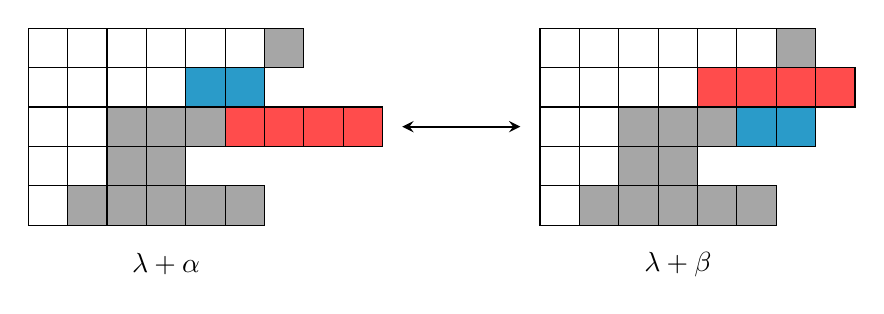
\begin{tikzpicture}[
                x=0.5cm, y=0.5cm,
                square/.style={draw, minimum size=0.5cm},
                white/.style={fill=white},
                gray/.style={fill=gray!70},
                blue/.style={fill=cyan!80!black},
                green/.style={fill=green!80!black},
                red/.style={fill=red!70!white}
            ]
            \begin{scope}[shift={(0,0)}]
                % First Row
                \foreach \x in {0,1,2,3,4,5} { \node[square, white] at (\x,4) {}; }
                \node[square, gray] at (6,4) {};
    
                % Second Row
                \foreach \x in {0,1,2,3} { \node[square, white] at (\x,3) {}; }
                \foreach \x in {4,5} { \node[square, blue] at (\x,3) {}; }
    
                % Third Row
                \foreach \x in {0,1} { \node[square, white] at (\x,2) {}; }
                \foreach \x in {2,3,4} { \node[square, gray] at (\x,2) {}; }
                \foreach \x in {5,6,7,8} { \node[square, red] at (\x,2) {}; }
    
                % Fourth Row
                \foreach \x in {0,1} { \node[square, white] at (\x,1) {}; }
                \foreach \x in {2,3} { \node[square, gray] at (\x,1) {}; }
    
                % Fifth Row
                \node[square, white] at (0,0) {};
                \foreach \x in {1,2,3,4,5} { \node[square, gray] at (\x,0) {}; }
            \end{scope}
            \node at (3, -1.5) {$\lambda + \alpha$};
            \begin{scope}[shift={(13,0)}] % Position of the second grid
                % First Row
                \foreach \x in {0,1,2,3,4,5} { \node[square, white] at (\x,4) {}; }
                \node[square, gray] at (6,4) {};
    
                % Second Row
                \foreach \x in {0,1,2,3} { \node[square, white] at (\x,3) {}; }
                \foreach \x in {4,5,6,7} { \node[square, red] at (\x,3) {}; }
    
                % Third Row
                \foreach \x in {0,1} { \node[square, white] at (\x,2) {}; }
                \foreach \x in {2,3,4} { \node[square, gray] at (\x,2) {}; }
                \foreach \x in {5,6} { \node[square, blue] at (\x,2) {}; }
    
                % Fourth Row
                \foreach \x in {0,1} { \node[square, white] at (\x,1) {}; }
                \foreach \x in {2,3} { \node[square, gray] at (\x,1) {}; }
    
                % Fifth Row
                \node[square, white] at (0,0) {};
                \foreach \x in {1,2,3,4,5} { \node[square, gray] at (\x,0) {}; }
            \end{scope}
            \node at (16, -1.5) {$\lambda + \beta$};
            \draw[<->, thick, >=stealth] (9,2) -- (12,2) node[midway, above] {};
    
        \end{tikzpicture}
        \caption{Example of the involution in the proof of Pieri's \(h\)-formula.}
        \label{fig:pieri-h-formula-involution}
    \end{figure}
    
    This map from \(\mathcal{B}\) to itself is an involution,
    and it satisfies that
        \(\lambda + \alpha + \delta_n\)
        \(\lambda + \beta + \delta_n\)
    differ by one transposition,
    hence
    \begin{equation}
        \tilde{a}_{\lambda + \alpha + \delta_n} + \tilde{a}_{\lambda + \beta + \delta_n} = 0.
    \end{equation}
    Finally,
    this implies that
    \begin{equation}
        \sum_{\alpha \in \mathcal{B}}
        \tilde{a}_{\lambda + \alpha + \delta_n}
        = 0,
    \end{equation}
    and consequently
    \begin{align}
        \tilde{a}_{\lambda + \delta_n} h_k
        &= \sum_{\substack{\text{compositions } \alpha \\ \text{of } k \text{ with length } n \\ (\lambda + \alpha) \setminus \lambda \text{ is a horizontal strip}}}
        \tilde{a}_{\lambda + \alpha + \delta_n} \\
        &= \sum_{\substack{\text{partitions } \mu \\ \lambda \setminus \mu \text{ is a Horizontal strip of size } k}}
        \tilde{a}_{\mu + \delta_n}.
    \end{align}
    Therefore,
    \begin{equation}
        a_\lambda h_k = \sum_{\mu} a_{\mu},
    \end{equation}
    where the sum is over all partitions \(\mu\) obtained by adding a horizontal strip of size \(k\) to \(\lambda\).
    Finally, the result follows by dividing by \(v_n\).
\end{proof}